\section{Versuchsdurchführung}

\subsection{Aufnahme der \textgamma-Spektren und des Untergrunds}
Der NaI-Szintillationszähler wird, wie auf \autoref{img:aufbau} gezeigt, über den Verstärker mit
dem MCA verbunden.
Um den passenden Verstärkungsfaktor für den Verstärker zu finden, wird die Thoriumprobe verwendet
und die Verstärkung so eingestellt, dass der höchste sichtbare Peak bei Kanal 6500 des MCA liegt.
Die Grobverstärkung beträgt dann 20, die Feinverstärkung 5.5. Als \emph{shaping time} wird 2\,\textmu s verwendet.
Die \emph{lower level discrimination}, die zur Verringerung der Totzeit des MCAs den unteren Teil des
Spektrums abschneidet, wird für alle folgenden Messungen auf 1 \% gestellt.\\
Mit diesem Aufbau werden für je 30 Minuten die Spektren von ${}^{22}$Na, ${}^{60}$Co und ${}^{152}$Eu aufgenommen.
Die Proben werden dazu in eine Bleiabschirmung direkt vor den Szintillationszähler gestellt\footnote{Für die
Messung von Natrium muss ein geringfügig anderer Aufbau ohne Bleiabschirmung verwendet werden,
da die passende Natriumprobe nicht mehr genügend Aktivität besitzt.
Die Messungen sind daher nur eingeschränkt vergleichbar.
Da hier aber nur die Position der Peaks von Interesse ist, stellt dies kein Problem dar.}.
Aus einem Loch in der Abschirmung gelangt Strahlung in den Zähler.
Mit den so gewonnenen Daten ist es möglich, eine Energieeichung des MCA durchzuführen.
(Die Zuordnung der Energien zu den Kanälen das MCA ist abhängig vom  Verstärkungsfaktor am Verstärker.
Zwischen den Experimente darf die Verstärkung deswegen auf keinen Fall geändert werden.)\\
Anschließend wird für 15 Stunden lang über Nacht mit leerer Bleiabschirmung die Untergrundstrahlung bestimmt.
Die Messung an ${}^{228}$Th wird mit dem selben Aufbau 64~Stunden lang über das Wochenende durchgeführt.



\subsection{Koinzidenzmessung}

Da für die Messung der Koinzidenzen eine sehr genaue Einstellung der Geräteparameter notwendig ist,
wird zunächst mit dem Oszilloskop das Signal an einzelnen Punkten der Schaltung beobachtet,
um dann die passenden Einstellungen zu finden.\\
\autoref{img:najunip} zeigt das Ausgangssignal des NaI-Szintillators und das verstärkte unipolare Signal,
das (in diesem Versuchsteil durch das \emph{gate}) in den MCA gelangt.
Die Länge des Szintillatorsignals beträgt für das hier registrierte \textgamma-Photon ca.~1\,\textmu s,
seine Amplitude etwas mehr als 200\,mV.
Die Amplitude des verstärkten Signals beträgt ca.~2.5\,V,
sein Maximum liegt 120\,ns nach dem Einsatzpunkt des Szintillatorsignals.

\begin{figure}[H]
\begin{center}
  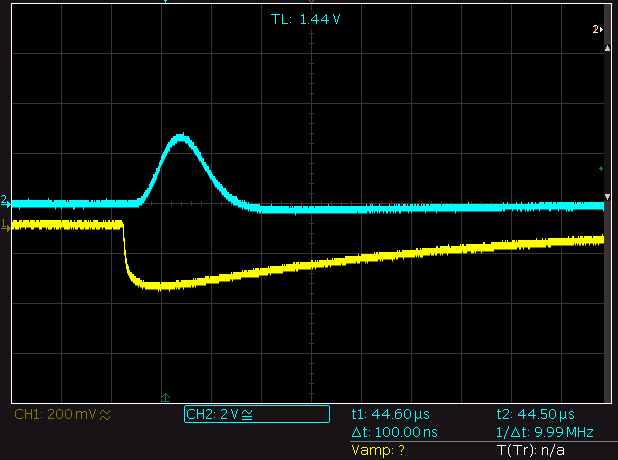
\includegraphics[width=0.65\textwidth]{../img/SCR0013.PNG}
  \caption[---]{Ausgangssignal des NaI-Szintillators (gelb) und Signal am unipolaren Ausgang des Verstärkers (blau).}
  \label{img:najunip}
\end{center}
\end{figure}

\autoref{img:najbiptu} zeigt ebenfalls ein Signal des NaI-Kristalls,
dann aber das verstärkte Signal am \emph{bipolaren} Ausgang des Verstärkers.
Man erkennt, dass das Maximum des bipolaren Signals schneller erreicht ist als das des unipolaren Signals;
der Abstand zum Einsatz des Szintillatorsignals beträgt hier nur 80\,ns (dies liegt daran,
dass das bipolare Signal die Ableitung des Unipolaren ist und bereits am Wendepunkt des Unipolaren sein Maximum
annimmt).\\
Das bipolare Signal wird mit dem Eingang des SCAs verbunden und dort zu einem Rechteckspuls geformt.
Da der Puls noch nicht schön geformt ist, bekommt er in der \emph{timing unit} eine schönere Form und eine Länge von
20\,ns. Dieser Puls ist auch auf \autoref{img:najbiptu} gezeigt.
\autoref{img:najbipsca2} zeigt die gleichen Signale in größerer Auflösung.
Hier lässt sich die zeitliche Verzögerung zwischen Einsetzen des Szintillatorsignals und Rechteckspuls
gut ablesen: Sie beträgt 135\,ns.

\begin{figure}[H]
\begin{center}
  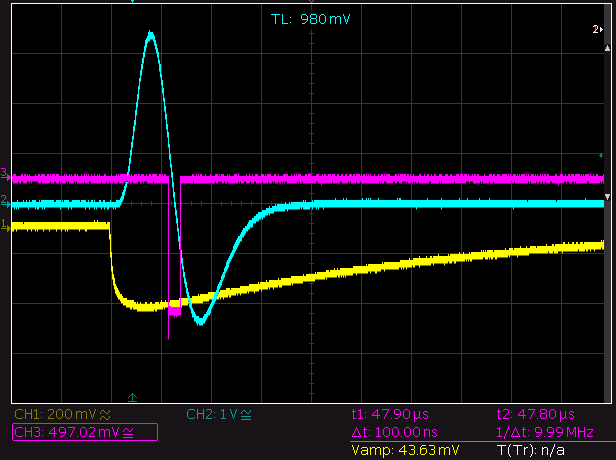
\includegraphics[width=0.65\textwidth]{../img/SCR0023.PNG}
  \caption[---]{Ausgangssignal des NaI-Szintillators (gelb),
  Signal am bipolaren Ausgang des Verstärkers (blau)
  und Rechteckspuls nach der \emph{timing unit} (rosa).}
  \label{img:najbiptu}
\end{center}
\end{figure}

\begin{figure}[H]
\begin{center}
  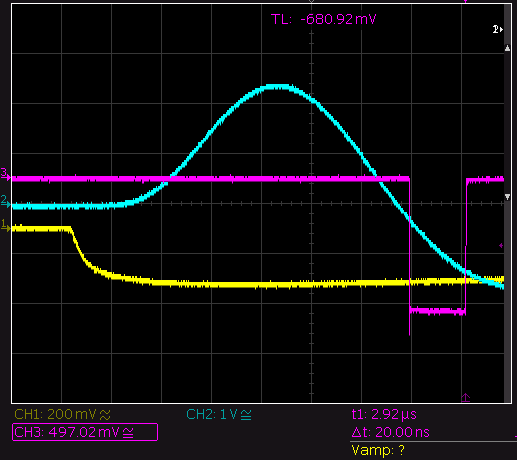
\includegraphics[width=0.65\textwidth]{../img/SCR0025.PNG}
  \caption[---]{Vergrößerter Ausschnitt aus \autoref{img:najbiptu} zur Bestimmung der Zeitverzögerung zwischen
  Einsatz des Szintillatorsignals (gelb) und Rechteckspuls (rosa) (135\,ns).}
  \label{img:najbipsca2}
\end{center}
\end{figure}

\begin{figure}[H]
\begin{center}
  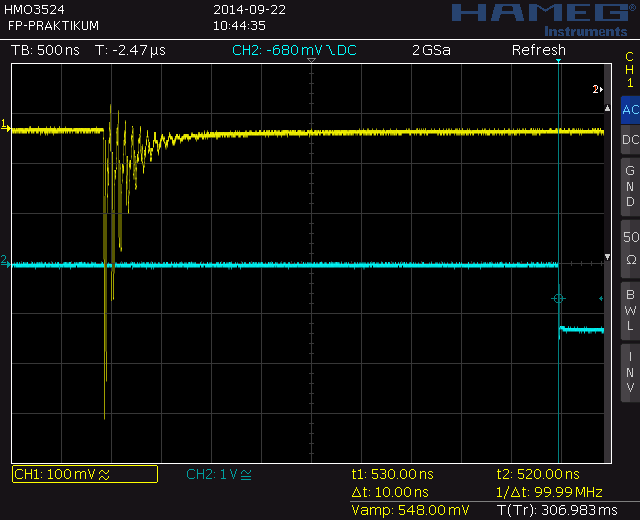
\includegraphics[width=0.65\textwidth]{../img/SCR0049.PNG}
  \caption[---]{Ausgangssignal des Plastik-Szintillators (gelb) und
  Rechteckspuls nach der \emph{timing unit} (blau) zur Bestimmung der Zeitverzögerung (90\,ns).}
  \label{img:plastiktu}
\end{center}
\end{figure}


Analog zum Anschluss der Geräte nach dem NaI-Szintillator wird der gleiche Aufbau nach dem Plastikszintillator
aufgebaut. Das Signal des Plastikszintillators ist auf \autoref{img:plastiktu} zu sehen:
Im Vergleich zum NaI-Szintillator ist die Amplitude hier viel höher (ca.~3\,V),
die Signallänge beträgt aber nur wenig mehr als 10\,ns.\\
Als Verstärkungsfaktor am Verstärker nach dem Plastik-Szintillator wurde auf 10\,$\cdot$\,100 eingestellt.
Die Überlegung dafür war folgende: Die Verstärkung sollte möglichst hoch sein,
um auch kleine Signale noch zu registrieren.
Eine zu hohe Verstärkung führt allerdings dazu, dass auch zufälliges Rauschen als Ereignisse gezählt wird.
Die geeignete Verstärkung wurde mit kurzen Probemessungen gefunden.
\autoref{tab:probemessung} zeigt die Messergebnisse.
\begin{table}[H]
\caption{Probemessungen mit dem Plastik-Szintillator zur Einstellung der geeigneten Verstärkung.}
\begin{center}
\begin{tabular}{|c|c|c|}
  \hline
  Verstärkung & Winkel & Ereignisse \\ \hline
  1000 & 90$^\circ$ & 2  \\ \hline
  1000 & 180$^\circ$ & 34  \\ \hline
  2000 & 90$^\circ$ & 9  \\ \hline
  2000 & 180$^\circ$ & 48  \\ \hline
\end{tabular}
\end{center}
\label{tab:probemessung}
\end{table}
Die Messdauer betrug jeweils 100\,s.
Bei einer Winkeleinstellung von 90$^\circ$ werden nur zufällige Koinzidenzen
des Untergrunds gemessen, bei 180$^\circ$ auch Ereignisse, die aus der Annihilation von Elektronen
und Positronen stammen.
(Der weitere Messaufbau nach den Verstärkern zur Registrierung der Koinzidenzen wird unten beschrieben.)\\
Die kurzen Messzeiten führen natürlich zu hohen relativen Fehlern auf die Messwerte,
vor allem bei geringer Zahl der Messereignisse.
Da hier aber nur eine geeignete Verstärkung für die späteren Messungen abgeschätzt werden soll,
wird auf eine Fehlerbetrachtung verzichtet.
Aus den Verhältnissen von Messsignal zum Untergrund kann für beide Messungen das
Signal-zu-Rausch-Verhältnis berechnet werden:
\begin{equation}
  \begin{split}
  \text{SRV}_{1000} & = \frac{34-2}{2} = 16 \\
   \text{SRV}_{2000} & = \frac{48-9}{9} = 4.3
  \end{split}
\end{equation}
Ein Vergleich der beiden Werte zeigt, warum der Verstärkungsfaktor 1000 für die weiteren Messungen gewählt wird.\\[\baselineskip]
Wie bei dem NaI-Szintillator wird das bipolare Ausgangssignal des Verstärkers in einen SCA
und dann in die \emph{timing unit} geleitet.
Der Rechteckspuls nach der \emph{timing unit} ist ebenfalls auf \autoref{img:plastiktu} zu sehen.
Er kommt hier schneller an als beim anderen Szintillator, 
die Laufzeit beträgt nur 90\,ns. Dieser Laufzeitunterschied wird dann am SCA mit der
Einstellung für das \emph{delay} auf 135\,ns verlängert (Erhöhung von 0 auf 3.05),
so dass zwei Signale, die von der selben
Elektron-Positron-Annihilation stammen, auch gleichzeitig an der Koinzidenzeinheit eintreffen.\\
Hier liegt eine weitere kritische Einstellmöglichkeit der Schaltung:
Die Koinzidenzeinheit liefert einen Puls an den Zähler, wenn an ihr zwei Rechteckspulse eintreffen,
die eine zeitliche Überschneidung besitzen.
Die Laufzeit der Signale, die für beide Szintillatoren auf 135\,ns eingestellt wurde,
schwankt allerdings um ca. 5\,ns. Wird an der \emph{timing unit}
die Breite der Rechteckspulse zu gering eingestellt, so
kann es sein, dass sie sich an der Koinzidenzeinheit nicht überschneiden und somit fälschlicherweise nicht
gezählt werden. Ist die Pulsbreite zu hoch, so werden sehr viele zufällige Koinzidenzen registriert.
Die Pulsbreite von 20\,ns erwies sich als optimal.\\
\autoref{img:koinzidenzen} zeigt Signale, die an der Koinzidenzeinheit ankommen:
Die Pulse, die in der Mitte der Abbildung liegen, sind koinzident.
Das Signal am rechten Rand ist zufällig, aber weit genug entfernt, um nicht registriert zu werden.
\begin{figure}[H]
\begin{center}
  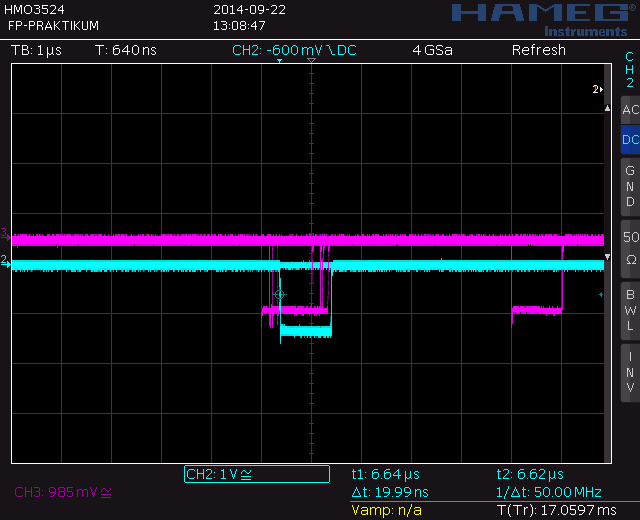
\includegraphics[width=0.65\textwidth]{../img/SCR0059.PNG}
  \caption{Eingangssignale an der Koinzidenzeinheit: Sich überschneidende Rechteckspulse werden als 
  Koinzidenzen registriert. Der Puls am rechten Rand ist zufällig und wird nicht registriert.}
  \label{img:koinzidenzen}
\end{center}
\end{figure}
Um die Anzahl der zufälligen Koinzidenzen zu verringern
und den Messaufbau empfindlicher für die Vernichtungsphotonen mit einer Energie von 511\,keV zu machen,
wird die Tatsache genutzt, dass mit den vorherigen Messungen bereits eine Möglichkeit zur
Energiemessung der Photonen im NaI-Szintillationszähler vorliegt.
Wie bei der 1. Messung wird am Computer das Messsignal des MCA beobachtet.
Wird nun am SCA die obere und die untere Schwelle geändert, so lassen sich ihre Positionen
am Computer verfolgen, da das \emph{gate} nur Signale passieren lässt, die auch den SCA passieren.
Der SCA wird im \emph{window mode} betrieben, die untere Schwelle wird auf 1.3 und das Fenster auf 3.0 gestellt.
Die Signale, die dann am MCA ankommen, bilden den 511\,keV-Peak.
Nur diese Signale werden vom negativen Ausgang des SCA an die \emph{timing unit} weitergegeben.\\
Tabelle \autoref{tab:params} gibt einen zusammenfassenden Überblick über die Einstellungen der Geräte.
\begin{table}[H]
\caption{Einstellungen an den Geräten für die Koinzidenzmessung.}
\begin{center}
\begin{tabular}{|c|c|c|}
  \hline
  \multicolumn{3}{|l|}{\textbf{NaI-Verstärker}} \\ \hline  
  Verstärkung & \multicolumn{2}{|c|}{shaping time} \\ \hline
  5.5\,$\cdot$\,20 = 110 & \multicolumn{2}{|c|}{20\,\textmu s}   \\ \hline
   \multicolumn{3}{|l|}{\textbf{NaI-SCA}} \\ \hline  
  lower threshold & window & delay \\ \hline
  1.3 & 3.0 & 0  \\ \hline
  \multicolumn{3}{|l|}{\textbf{Plastik-Verstärker}} \\ \hline  
  Verstärkung & \multicolumn{2}{|c|}{shaping time}   \\ \hline
  10\,$\cdot$\,100 = 1000 & \multicolumn{2}{|c|}{20\,\textmu s}  \\ \hline
   \multicolumn{3}{|l|}{\textbf{Plastik-SCA}} \\ \hline  
  lower threshold & upper threshold & delay \\ \hline
  min & max & 3.05  \\ \hline
     \multicolumn{3}{|l|}{\textbf{timing unit}} \\ \hline  
  \multicolumn{3}{|c|}{Signallänge}   \\ \hline
  \multicolumn{3}{|c|}{20\,ns}   \\ \hline
 
\end{tabular}
\end{center}
\label{tab:params}
\end{table}
Nach Anschluss und Einstellung der Geräte wird die Koinzidenzmessung an $^{22}$Na durchgeführt.
Dazu werden acht 1000\,s lange Messungen in 5$^\circ$-Schritten um das Maximum der Intensität bei 180$^\circ$
durchgeführt sowie zwei genauso lange Untergrundmessungen, bei denen die Szintillatoren im rechten Winkel
zueinander stehen.